\documentclass{ximera}

\input{preamble.tex}

\author{Gregory Hartman \and Matthew Carr}
\license{Creative Commons 3.0 By-NC}
\acknowledgement{https://github.com/APEXCalculus}

\begin{document}
\begin{exercise}

\outcome{Calculate limits using the limit laws.}
\outcome{Calculate limits of piecewise functions.}

\tag{limit} 
\tag{piecewise} 
\tag{continuous}
\tag{trigonometric}

  Find 
  \[
  \lim_{x\to 0} f(x)
  \begin{prompt}
  = \answer{1}.
  \end{prompt}
  \]
  where
  \[
  f(x) = \left\{\begin{array}{cl} \cos(x) & x\leq 0, \\ x^2+3x+1 & x>0. \end{array}\right.
  \]
    \begin{hint}
     Both pieces of $f(x)$, $\cos(x)$, for $x\leq0$, and $x^2+3x+1$, for $x>0$, are continuous for all $x$. However, for the limit $\lim_{x\to0}f(x)$ to exist, both the left-hand and the right-hand limits of $f(x)$ at $0$ must exist and be equal.
    \end{hint}
     \begin{hint}
    	Take a look at the graph of the function
    \begin{center}
     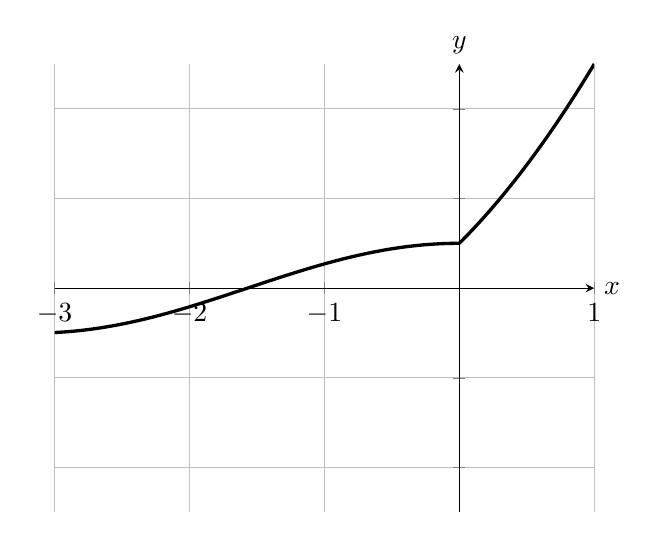
\begin{tikzpicture}
	\begin{axis}
	[ymin=-5,ymax=5, axis lines=center,xlabel=$x$,ylabel=$y$,every axis y 
	label/.style={at=(current axis.above origin),anchor=south},every axis x label/.style={at=(current axis.right of origin),anchor=west},
	domain=-5:5,
	yticklabels={},
	ymajorgrids=true,
	grid = major
	]
	\addplot[domain=-3:1,very thick,smooth,samples=1000]
	{(!(\x>0))*(cos(deg(\x)))+(\x>0)*(\x^2+3*\x+1)};
	\end{axis}
       \end{tikzpicture}      
      \end{center} 
    \end{hint}
    \begin{hint}
     Evaluating $\lim_{x\to0^{+}}f(x)$ we see that it is $1$. This follows because for $x>0$, we are on the piece of $f(x)$ given by $x^2+3x+1$ and the limit $\lim_{x\to0}\left({x^2+3x+1}\right)=\left({\lim_{x\to0}(x)}\right)^2+3\cdot\lim_{x\to0}(x)+\lim_{x\to0}\left({1}\right)=1$, certainly. On the other hand, evaluating $\lim_{x\to0^{-}}f(x)$ we see it is equal to $1$. This follows because, for $x\leq0$, we are on the piece of $f(x)$ given by $\cos(x)$ and the limit $\lim_{x\to0}\cos(x)=1$, certainly. These are equal, so the limit exists and is equal to $1$.
    \end{hint}
\end{exercise}

\end{document}